\section{پردازشگر‌های زبان}
\begin{frame}[fragile]{پردازش‌گر‌های زبان}
\begin{itemize}\itemr
\item[-]
به بیان ساده، کامپایلر برنامه‌ایست که می‌تواند یک برنامه را با یک زبان (\lr{\textit{source} language}) بخواند، و معادل آن را به زبانی دیگر ترجمه کند  (\lr{\textit{targer} language}.)
\vspace{5mm}
\begin{figure}[H]
\begin{center}
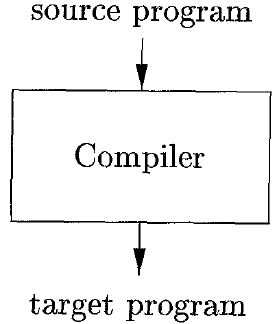
\includegraphics[width=0.3\textwidth, height=0.6\textheight, angle=1]{docs/images/sct}
\end{center}
\end{figure}
\end{itemize}
\end{frame}

\begin{frame}{برنامه‌ی ترجمه شده}
\begin{itemize}\itemr
\item[-]
اگر برنامه‌ی تولید شده، یک 
\lr{executable machine-language program}
باشد، می‌توان آن را مستقیما توسط پردازنده اجرا کرد.
\vspace{5mm}
\begin{figure}[H]
\begin{center}
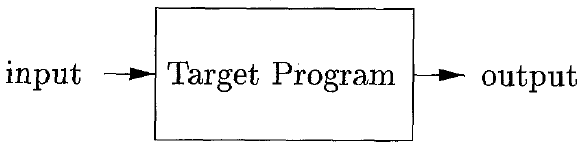
\includegraphics[width=0.6\textwidth, height=0.3\textheight, angle=0.5]{docs/images/executable}
\end{center}
\end{figure}
\end{itemize}
\end{frame}

\begin{frame}{مفسر}
\begin{itemize}\itemr
\item[-]
نوع دیگری از پردازش‌گر‌های زبانی، مفسرها هستند که بجای تبدیل زبان به زبان دیگر (\lr{\textit{target}})، خود مستقیما مسئول اجرای زبان اول (\lr{\textit{source}}) می‌شوند.
\vspace{5mm}
\begin{figure}[H]
\begin{center}
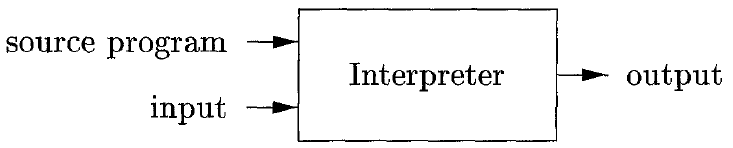
\includegraphics[width=0.7\textwidth, height=0.3\textheight, angle=0]{docs/images/interpreter}
\end{center}
\end{figure}
\end{itemize}
\end{frame}

\begin{frame}{یک سیستم پردازشگر زبان - \lr{Preprocessor}}
\begin{figure}[H]
\begin{center}
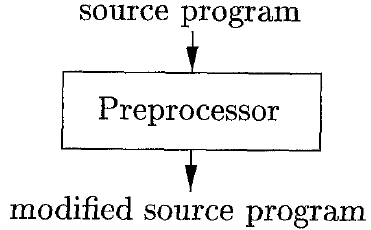
\includegraphics[width=0.5\textwidth, height=0.5\textheight, angle=0.6]{docs/images/preprocessor}
\end{center}
\end{figure}
\end{frame}

\begin{frame}[fragile]{\lr{Preprocessor}}
\begin{itemize}\itemr
\item[-]<1->
زبان‌های کهنی مثل \lr{C} و \lr{C++} سیستم \lr{moduling} و ساختاربندی منظمی برای جدا کردن \lr{source code}هایشان نداشتند.

\item[-]<2->
اما زبان‌های جدیدتر مثل \lr{Python} چنین سیستمی را دارند.

\begin{latin}
\begin{lstlisting}[language=python]
import math
from csv import reader, writer
\end{lstlisting}
\end{latin}
\end{itemize}
\end{frame}

\begin{frame}{\lr{Preprocessor}}
\begin{itemize}\itemr
\item[-]<1->
به همین دلیل، آنها نیاز داشتند که وقتی برنامه‌ای که نوشته‌اند را به چندین فایل تقسیم کرده‌اند، کامپایل کنند، برنامه‌ای تمام \lr{source code}هایشان را به یک 
\lr{source code}
واحد تبدیل کرده و آن را به کامپایلر بدهند، که بخاطر این نیاز، نرم‌افزاری به نام 
\lr{Preprocessor}
نوشته شد.
\end{itemize}
\end{frame}

\begin{frame}{\lr{Preprocessor}}
\begin{figure}[H]
\begin{center}
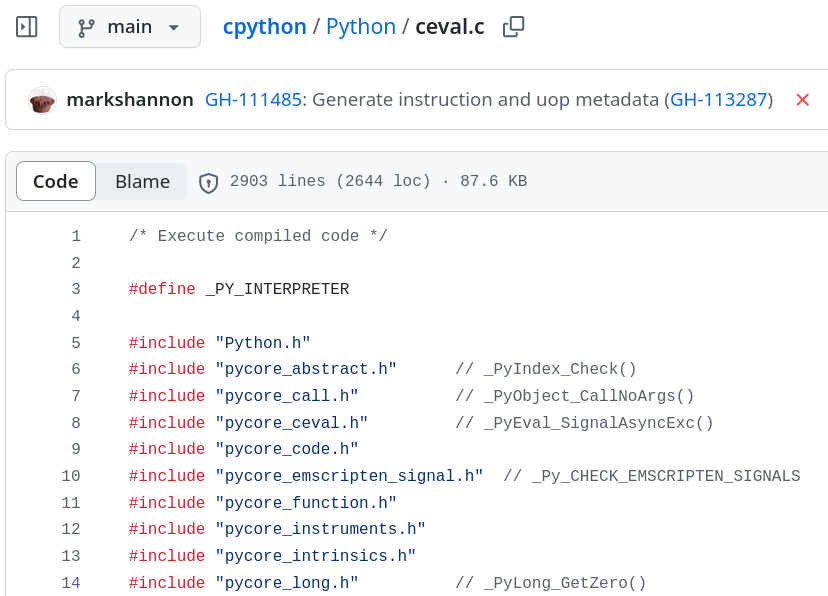
\includegraphics[width=0.6\textwidth, height=0.7\textheight]{docs/images/include}
\end{center}
\end{figure}
\end{frame}

\begin{frame}{\lr{Preprocessor}}
\begin{itemize}\itemr
\item[-]
با \lr{Preprocessor}ها می‌توان ماکرو به زبان اضافه کرد.

\vspace{5mm}
\begin{figure}[H]
\begin{center}
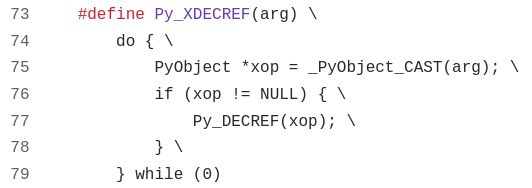
\includegraphics[width=0.7\textwidth, height=0.5\textheight]{docs/images/define}
\end{center}
\end{figure}
\end{itemize}
\end{frame}

\begin{frame}{یک سیستم پردازشگر زبان - \lr{Compiler}}
\begin{figure}[H]
\begin{center}
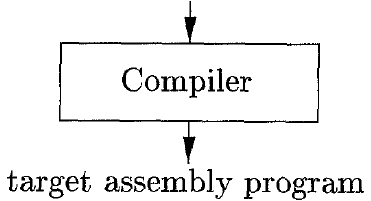
\includegraphics[width=0.5\textwidth, height=0.5\textheight, angle=0.6]{docs/images/compiler}
\end{center}
\end{figure}
\end{frame}

\begin{frame}{یک سیستم پردازشگر زبان - \lr{Assembler}}
\begin{figure}[H]
\begin{center}
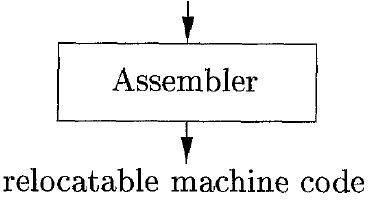
\includegraphics[width=0.5\textwidth, height=0.5\textheight, angle=0.6]{docs/images/assembler}
\end{center}
\end{figure}
\end{frame}

\begin{frame}{یک سیستم پردازشگر زبان - \lr{Linker/Loader}}
\begin{figure}[H]
\begin{center}
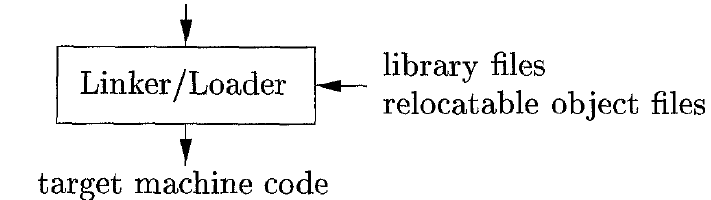
\includegraphics[width=0.75\textwidth, height=0.5\textheight, angle=0.4]{docs/images/linkerloader}
\end{center}
\end{figure}
\end{frame}